\section{Installation of Python and Miniconda}
\label{appendix:second}

Installation of the software for programming in Python on a computer is easiest with a \emph{package manager}. The recommended package manager for Python is named \textsf{conda}. It can be used as a Windows console (\textsf{Anaconda Prompt}), which is very similar to the implementation in a Linux or MacOS X \textsf{bash} console. 
The console program is called \textsf{Miniconda} and can be downloaded at:

\url{https://docs.conda.io/en/latest/miniconda.html}. 
 
Miniconda is available for Windows, Linux and MacOS.
In general, nowadays, one would choose the latest Miniconda Python 3.x version 64-bit installer:\textsf{ Miniconda3-latest-Windows-x86\_64.exe} on Windows, or the analogous installers for Linux and MacOS X.

\begin{itemize}
	\item Download and execute your installer
	\item Install “Just for me”	and create C:\textbackslash Users\textbackslash $\langle username\rangle$\textbackslash miniconda3. Note: $\langle username\rangle$ should NOT contain spaces. Do not install Miniconda system-wide in the "C:\textbackslash Program Files" directory.
	\item Take default options for PATH and REGISTRY update
\end{itemize}

\subsection{Anaconda Prompt}
\label{appendix:anaconda}

After installation of Anaconda (Miniconda) the Windows Start Menu contains a new group "Anaconda3". A detailed view is shown below:

\begin{figure}[H]
	\centering
	\begin{subfigure}[b]{0.38\textwidth}
		\includegraphics[width=\textwidth]{Figures/Anaconda_Prompt.png}
		\caption{Anaconda Start Menu}
		\label{AnacondaMenu}
	\end{subfigure}
	\hfill
	\begin{subfigure}[b]{0.52\textwidth}
		\includegraphics[width=\textwidth]{Figures/AnacondaCommandWindow.png}
		\caption{Anaconda Prompt}
		\label{AnacondaPrompt}
	\end{subfigure}
	\caption{Anaconda (Miniconda) tools installed on Windows}
	\label{AnacondaTools}
\end{figure}

\begin{comment}
	
	\begin{figure}
		\centering
		\begin{minipage}[b]{0.4\textwidth}
			\includegraphics[width=\textwidth]{../images/Anaconda_Prompt.png}
			\caption{Anaconda Start Menu}
			\label{fig:1}
		\end{minipage}
		\hfill
		\begin{minipage}[b]{0.4\textwidth}
			\includegraphics[width=\textwidth]{../images/AnacondaCommandWindow.png}
			\caption{Anaconda Prompt}
			\label{fig:2}
		\end{minipage}
	\end{figure}
	
\end{comment}

The Start Menu entry "\textsf{Anaconda Prompt (miniconda3)}" will open a Windows Command Prompt ("MS-DOS window") with special properties. The current directory name (standard prompt) is preceded by \textsf{(base)}. This is the name of the default \textsf{conda} \emph{environment}.
The \textsf{(base)} environment is \emph{NEVER} used for code development. After installation of the package manager, it contains the latest version of the Python interpreter, which is kept up-to-date with the command:

\textsf{conda update -n base -c defaults conda}

The Python interpreter in the \textsf{(base)} environment may be used by other Windows programs, which will then ask you for the location of the default Python interpreter.

The standard location is: \textsf{C:\textbackslash Users\textbackslash $\langle username\rangle$\textbackslash miniconda3\textbackslash python.exe}.

\subsection{Conda configuration}
\label{appendix:config}

Before creating any dedicated environments, it is recommended to optimize the \textsf{conda} configuration \cite{stack_channels, stack_multiple}. In the previous command, the \textsf{conda} \emph{package} was updated in the \textsf{base} \emph{environment}. The package was read from the \textsf{defaults} \emph{channel}. Other channels exist, that often contain more up-to-date versions of important Python packages. The channel \textsf{conda-forge} is keeping a more recent copy of many packages, including the \textsf{opencv} package, which is a key package used for image analysis. Therefore we add:

\begin{itemize}
	\item \textsf{conda config --show} \qquad this shows the configuration file. Look for "channels:".

    \item \textsf{conda config --add channels conda-forge} \qquad this adds the conda-forge channel before the defaults channel (top of the list).

    \item \textsf{conda config --set channel\_priority strict} \qquad this guarantees that channel priority is maintained according to the list.
\end{itemize}

The config file now shows: \\
... \\
\textsf{channel\_priority: strict \\
	channels: \\
	- conda-forge \\
	- defaults} \\
...

See also: \\
\url{https://stackoverflow.com/questions/39857289/should-conda-or-conda-forge-be-used-for-python-environments} \\
\url{https://conda-forge.org/docs/user/tipsandtricks.html#using-multiple-channels} \\

\subsection{Conda environments}
\label{appendix:environments}

A dedicated environment can be made with the command:

%\sffamily
\textsf{conda create -n $\langle env\_name \rangle$ python=3.x}
%\normalfont

The next commands are:

\textsf{activate $\langle env\_name \rangle$}

\textsf{conda info --envs} or \textsf{conda info -e}: note the active environment with asterisk *

\textsf{conda install $\langle package\_name \rangle$}
or
\textsf{pip install $\langle package\_name \rangle$}

The result can be seen with: \textsf{conda list} : note the packages are all compatible with your Python version

The commands can be stored in a textfile:

\lstinputlisting[label=appendix:envlist,caption=Example textfile with conda commands for new environment, language=Python, linerange={1-100}]{../../environment.txt}

Environments are stored in the private directory of the user. On Windows: 
C:\textbackslash Users\textbackslash $\langle username\rangle$\textbackslash miniconda3\textbackslash envs 

On Linux: /home/$\langle username\rangle$/miniconda3/envs

\textbf{Note:} Code development or storage is NEVER done in C:\textbackslash Users\textbackslash $\langle username\rangle$\textbackslash miniconda3 NOR in any of its subfolders.

\subsection{Python from the console}
\label{appendix:console}

The \textsf{Anaconda Prompt} program on Windows is a specialized version of the general Windows \textsf{Command Prompt}, formerly known as "MS-DOS window" or "console". The advantage of \textsf{Anaconda Prompt} is that all file paths to the Miniconda installation are automatically set and that the prompt indicates the currently active Python environment. On Linux and MacOS, \textsf{Anaconda Prompt} is integrated in the command-line terminal. Thus \textsf{Anaconda Prompt} looks very similar on all operating systems.

Running a Python script in the console is as simple as:

\textsf{activate $\langle env\_name \rangle$}

\textsf{conda info --envs} or \textsf{conda info -e}: note the active environment with asterisk *

\textsf{cd $\langle repository\_root \rangle$}

\textsf{python $\langle script\_name \rangle$}

For an overview of Python command-line features, see:

\url{https://realpython.com/python-command-line-arguments/#the-command-line-interface}

\subsection{Python IDE}
\label{appendix:ide}

\subsubsection{Installation}

\begin{figure}[H]
	\centering
	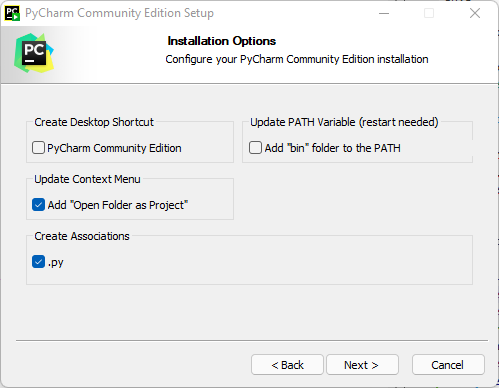
\includegraphics[width=0.5\textwidth]{Figures/PyCharm_checks.png}
	\caption{PyCharm IDE installation on Windows}
	\label{fig:PyCharm}
\end{figure}

After creation of the \textsf{conda} environment with the right selection of Python \emph{packages} for the analysis of the impedance measurements, it is recommended to develop the Python software in a dedicated IDE, where Python scripts can be edited, run, and debugged. The recommended program for this purpose is PyCharm, which can be downloaded here: 

\url{https://www.jetbrains.com/pycharm/download/#section=windows}

\url{https://www.jetbrains.com/community/education/#students}

\begin{itemize}
	\item Download the "Community" installer \textsf{pycharm-community-2021.3.2.exe} and run it.
	\item Install in default directory.
	\item Check options according to Figure~\ref{fig:PyCharm}.
	\item after succesful installation, navigate to the \emph{repository root} folder of your project and right-click on the canvas of the folder window (not on a file or subfolder icon). Choose the "Open Folder as PyCharm Project" item. The PyCharm IDE will start and open the project and subfolders.
	\item Once a project has been opened in PyCharm, it creates a (hidden) subfolder named \textsf{.idea} in the repository root folder. This folder contains the bookkeeping of the IDE. Do not change anything in this \textsf{.idea} subfolder. If anything goes wrong, delete it entirely, and PyCharm will create a fresh one.
	\item 
\end{itemize}

\begin{figure}[H]
	\centering
	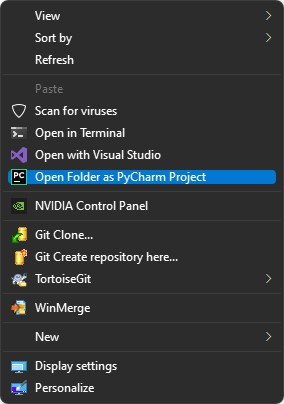
\includegraphics[width=0.3\textwidth]{Figures/context_menu_pycharm.jpg}
	\caption{PyCharm context menu after right-click on root folder canvas}
	\label{fig:contextmenu_pycharm}
\end{figure}

\subsubsection{Configuration}

\begin{itemize}
	\item To work with your Python code in PyCharm, you need to configure a Python interpreter. Assign the Python interpreter from your (existing!) \textsf{conda} environment created following the guidelines in Appendix \ref{appendix:environments} to the open project. In PyCharm,under File | Settings | Project | Project interpreter , the use of a dedicated project environment as default Python interpreter can be registered. This information is stored in the \textsf{.idea} hidden folder in the project root directory.
	
	See: \url{https://www.jetbrains.com/help/pycharm/configuring-python-interpreter.html}.
	
	\item After configuring the interpreter, the IDE needs some time to load all the packages from your environment. A progress bar is visible on the bottom of the IDE window.
\end{itemize}

\begin{figure}[H]
	\centering
	\begin{subfigure}[b]{0.45\textwidth}
		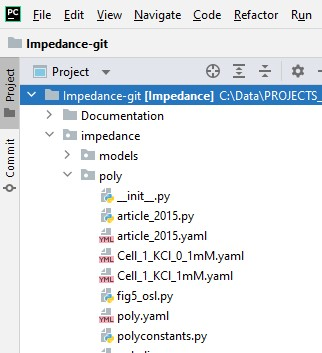
\includegraphics[width=\textwidth]{Figures/project_tab.jpg}
		\caption{Project tab with root folder and subfolders}
		\label{fig:pycharm_projecttab}
	\end{subfigure}
	\hfill
	\begin{subfigure}[b]{0.3\textwidth}
		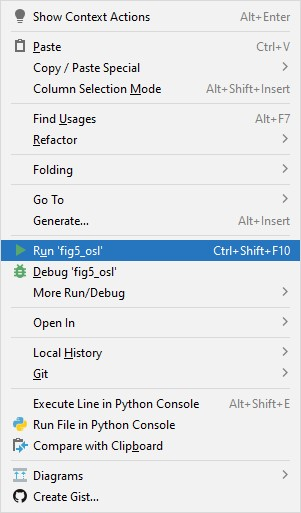
\includegraphics[width=\textwidth]{Figures/run.jpg}
		\caption{Context menu for right-click}
		\label{fig:pycharm_run}
	\end{subfigure}
	\caption{PyCharm project configuration and running}
	\label{fig:pycharm_config}
\end{figure}

\subsubsection{.gitignore}

Every Git repository has at least one \textsf{.gitignore} file in the repository root folder. This file contains a list of the files, folders and file-types which are NOT committed and pushed.

In the \textsf{.gitignore} file the following files/folders/file types are listed:

\begin{itemize}
	\item \textsf{.gitignore} itself. \textsf{.gitignore} is a LOCAL file which is not committed and pushed.
	\item The \textsf{.idea} folder. This is the local bookkeeping of PyCharm.
	\item The \_\_pycache\_\_ folders. Here, Python compiles code for local use. This causes your program to run faster after the first run.
\end{itemize}

Generally, using Python, only \textsf{*.py} or \textsf{*.ipynb} files are committed en pushed, plus some essential data and documentation.

\subsubsection{Running and debugging Python scripts}

The structure of a Python file (*.py-file, module) is as follows:

\begin{itemize}
	\item \textsf{import} statements
	\item executable code organized in functions (\textsf{def}) or classes (\textsf{class})
	\item the \textsf{\text{if \_\_name\_\_ == "\_\_main\_\_":}} clause. After this follows a validation of the functions / classes in the module.
\end{itemize}

This code pattern is essential for re-using the functions/classes in other Python modules. The pattern is recommended by Guido van Rossum, the inventor of the Python language.

\lstinputlisting[label=basic_py,caption={Basic structure of a Python module}, language=Python, linerange={1-100}]{./Listings/example.py}

\begin{itemize}
	\item Selecting a Python script in the Project tab can be done with a left-click. Right-clicking on a Python (*.py) module opens the context menu of Fig.~\ref{fig:pycharm_run}. Clicking the green arrow in the context menu starts executing the selected script.
	\item Double-clicking a *.py module in the Project tab opens the module in the editor window of the IDE. Right-clicking on the canvas of the editor window also opens the context menu of Fig.~\ref{fig:pycharm_run}.
\end{itemize}

\subsubsection{Python documentation}

Every function or class method contains a "docstring" directly after the def or class definition line. A docstring starts with """ en ends with """. It may consist of several lines of documentation. In PyCharm a docstring is automatically generated on typing """ at the appropriate location in the code.

\newpage